


We test $\varepsilon$-flatness by looking at direct simulation results from different starting points and see if they give roughly the same hitting probabilities. We further test whether the CHop probabilities agree with direct simulation results. Theorem \ref{thm:main_thm} shows that $\varepsilon$-flatness is valid, and CHop probabilities agree with global hitting probabilities in the limiting regime of small $r_A,r_B$, but it is not obvious whether the parameters we use lie in that regime.  In particular, we look at the case $r_A = 0.05, r_{\tilde{A}} = 0.1, r_B = 0.075, r_{\tilde{B}} = 0.15$. In this case, we see that the $\varepsilon$-flatness condition indeed holds, and the CHop probabiity yields an estimate for the hitting probability that is consistent with direct simulations:

\begin{description}
\item[Hitting probabilities estimated with direct simulations] $\approx 0.2236$. We run 2000 diffusion simulations at each one of the 100 randomly picked initial locations from $\mathcal{B}(0, 1) \setminus (\tilde{A} \cup \tilde{B})$. For each initial location we obtain an estimate of the hitting probability. The mean of these estimates is 0.2236, standard deviation 0.0093. We used time step of size 1e-05. A histogram of the different hitting probabilities, as well as the CHop probability, is shown in Fig. \ref{fig:simple_hitting_prob_test}. The hitting probabilities from different initial locations are in $[0.2055, 0.2480]$, and the $\varepsilon$-flatness condtion holds with $\varepsilon = 0.0425$.
  
\item[CHop probability]  0.2286, which is a good approximation for the various hitting probabilities we obtained from direct simulations.
\end{description}

\begin{figure}
	\caption{\label{fig:simple_hitting_prob_test} We picked 100 random locations for $ X_0 \not\in \mathcal{B}(0, 1) \setminus (\tilde{A} \cup \tilde{B})$. For each location we used 2000 simulations to estimate the probability of hitting $A$ before $B$. The histogram of the 100 estimates is shown below. The $\varepsilon$-flatness condtion holds with $\varepsilon = 0.0425,$ and the CHop probability gives good approximation to this narrow range of hitting probabilities.}
	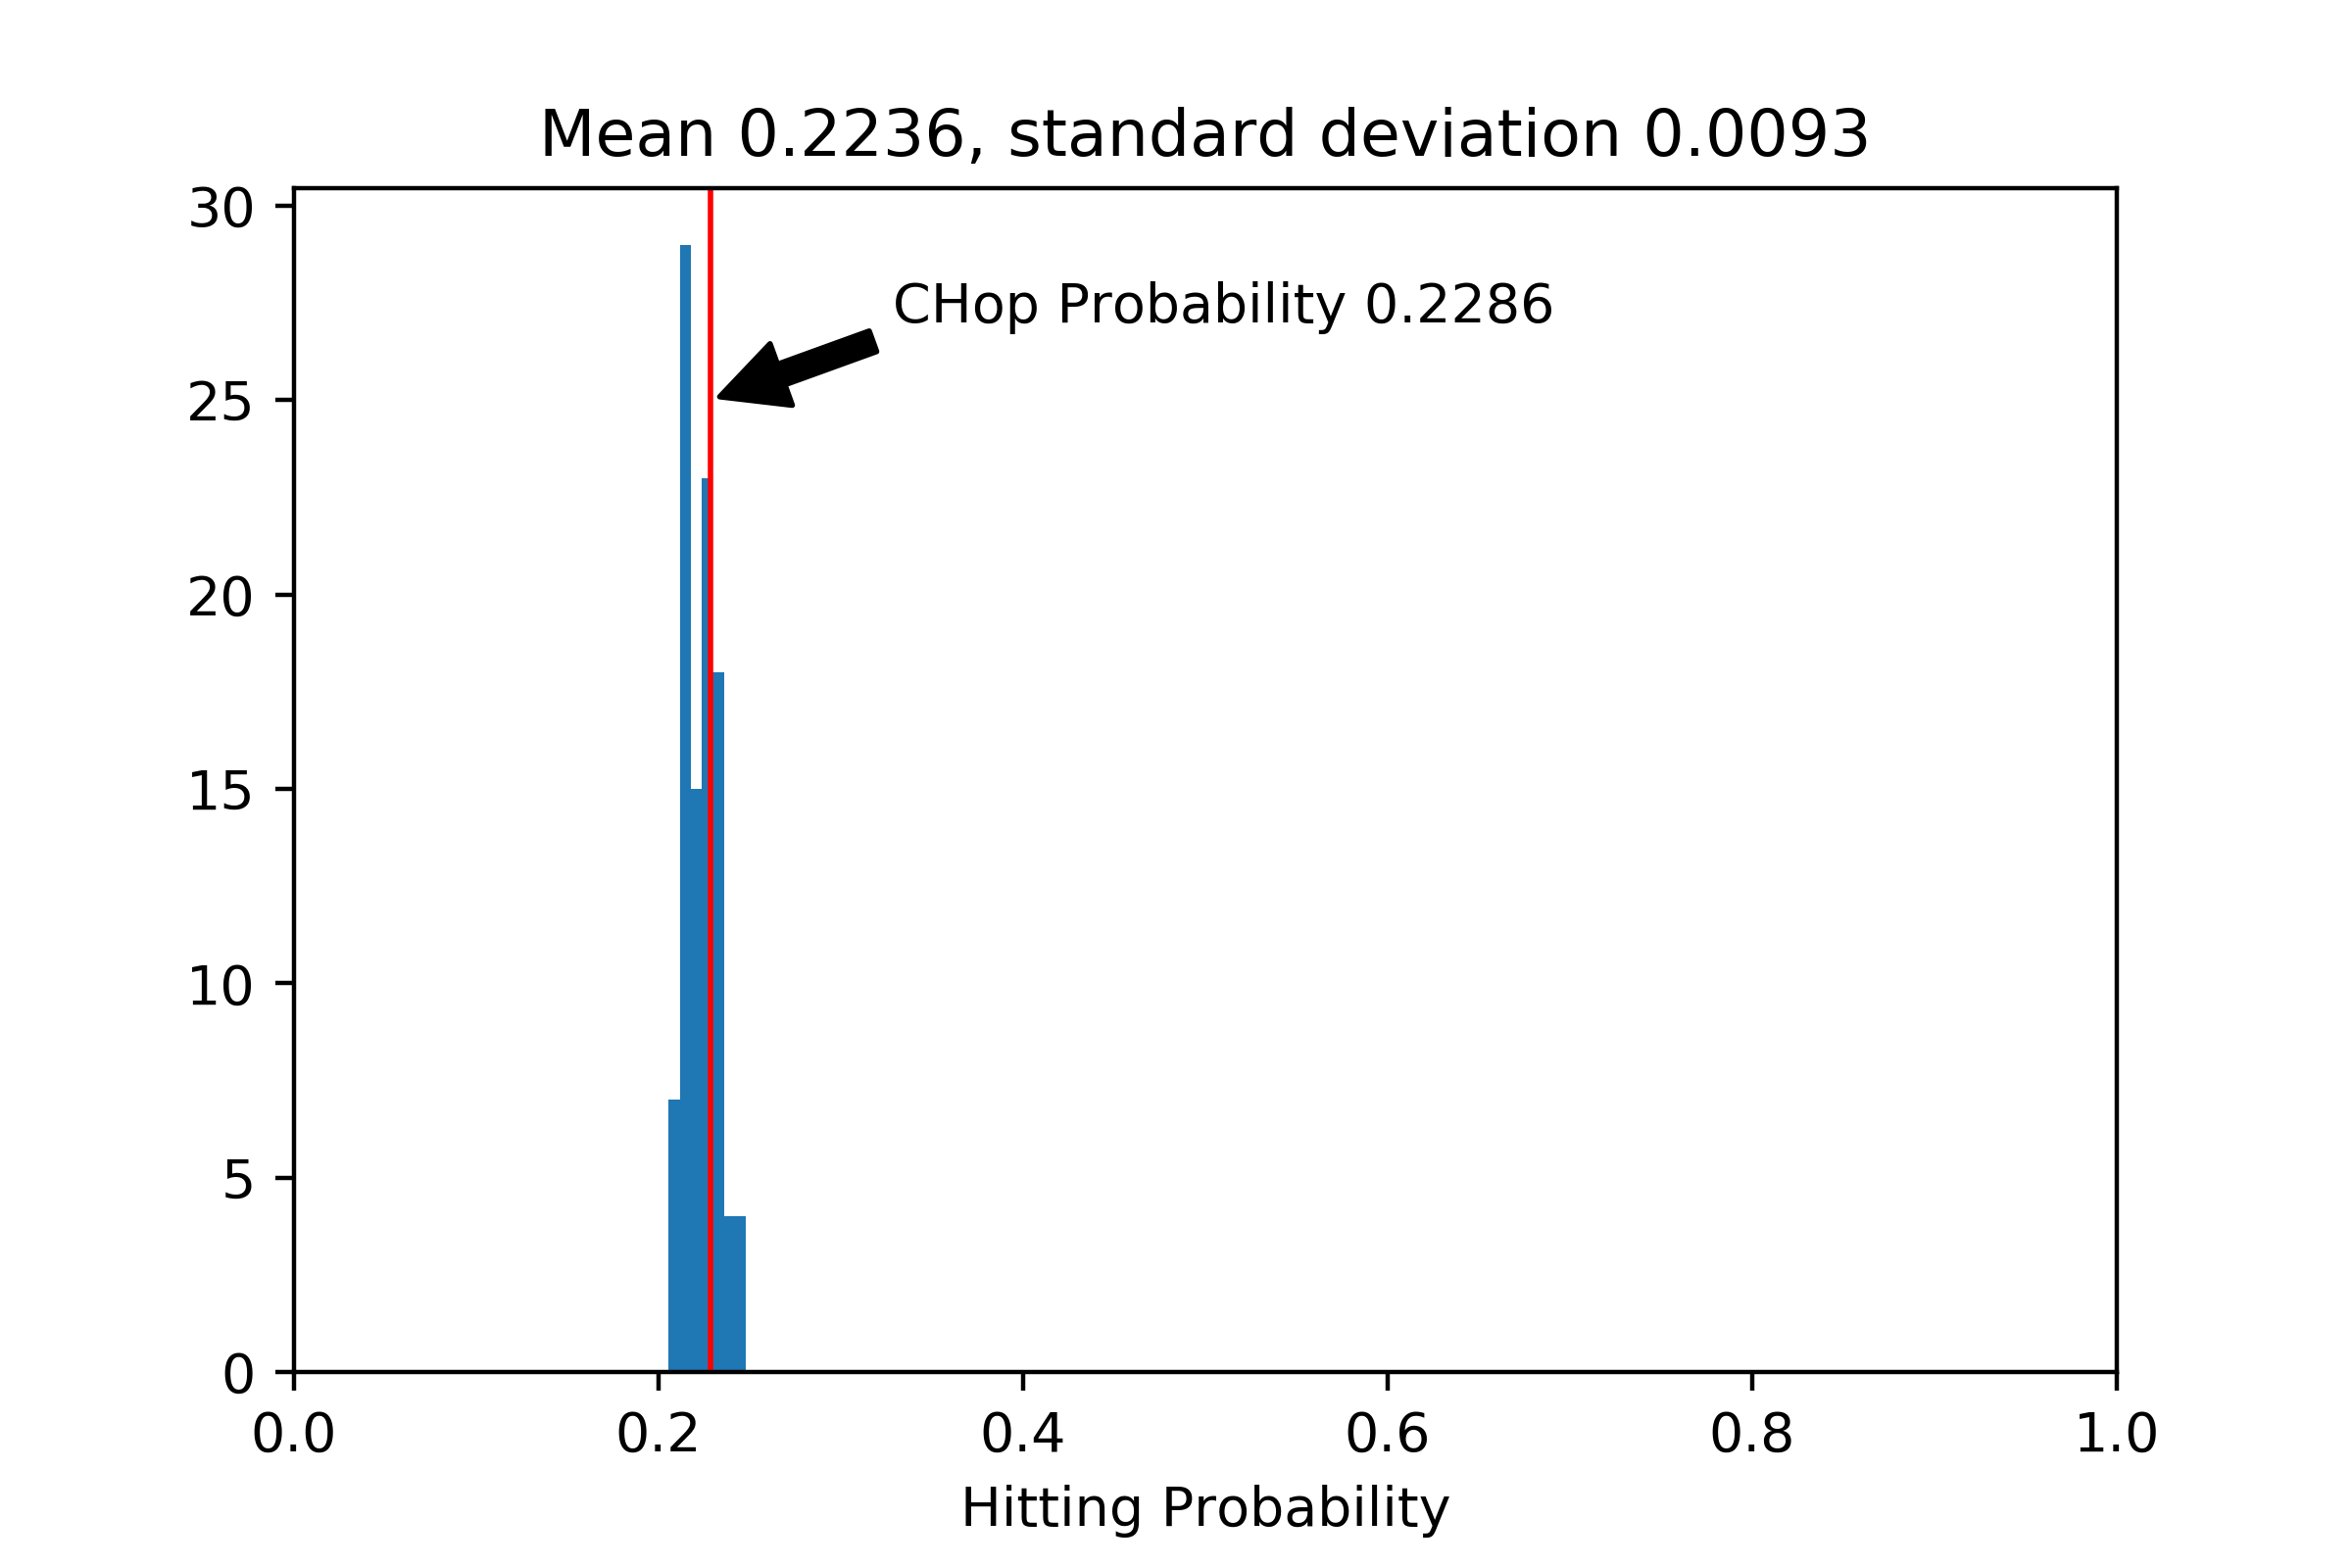
\includegraphics{figs/simple_hitting_prob_hist.png}
\end{figure}
